\chapter{Contribution}
\label{ch:contribution}

We pursue a neuro-symbolic pipeline for argumentation mining that leverages
probabilistic Answer Set Programming (PASP) as an expressive representation
language and compiles PASP programs into tractable circuits for efficient
inference. By embedding argumentative constraints into compiled circuits we aim
to align neural predictions with the semantics of bipolar argumentation,
enabling transparent reasoning, calibrated uncertainty, and scalable learning
loops.

\section{Scope and Roadmap}
\label{sec:contribution-roadmap}

This chapter is organised in four stages. Section~\ref{sec:problem-setting}
formalises the problem we study, first by explaining how textual argumentation
signals are mapped into PASP programs and then by detailing the knowledge
compilation pipeline that supports tractable inference. Section
\ref{sec:foundations} gathers the foundational notions we rely on: we introduce
the argumentation structures we model, recall Clark's completion, and discuss
the circuit properties we require from downstream compilers. The chapter closes
with Section~\ref{sec:experimental-outlook}, which anticipates the experimental
plan that will ultimately assess the proposed approach.

\section{Problem Setting}
\label{sec:problem-setting}

Before delving into the technical building blocks of our approach, we first
outline the problem setting we target and summarise the proposed pipeline for
scalable neuro-symbolic argumentation mining.

\subsection{From Argumentation Mining to PASP}

Argumentation mining systems must recognise argumentative spans, classify their
roles, and recover the interaction graph that ties them together
\citep{stab2017parsing}. Early neuro-symbolic pipelines coupled local neural
predictions with Integer Linear Programming constraints, whereas probabilistic
logic programming brought principled uncertainty handling to the task
\citep{fierens2015inference,manhaeve2018deepproblog,cerveira2023argumentation}. Stable
model semantics further broadens the expressiveness of these pipelines by
accommodating negative cycles and other non-monotonic phenomena that arise in
real discourse \citep{totis2023smproblog}.

We formalise an argumentation mining instance as a bipolar argumentation
framework whose nodes represent candidate arguments extracted from text and
whose labelled edges denote support or attack relations
\citep{toni2011argumentation, toni2023understanding}. Neural components provide
noisy observations—e.g.\ span detection probabilities or relational scores—that
we encode as probabilistic facts. The deterministic backbone of the PASP
program asserts domain constraints, propagates support chains, and enforces
well-formed argumentative structures. Inference tasks such as cautious or brave
reasoning over accepted arguments then reduce to answering PASP queries, which we
cast as instances of second-level algebraic model counting (2AMC)
\citep{kiesel2022efficient}.

\subsection{Knowledge Compilation Pipeline}
\label{sec:contribution:pipeline}

Directly solving these probabilistic programs on demand would be prohibitively
expensive. Instead, we adopt a knowledge compilation workflow that proceeds in
three stages: grounding, propositional rewriting, and circuit construction.
Grounding produces a finite propositional theory while retaining the structure
of the original program; propositional rewriting augments the theory with loop
formulas and other constraints that guarantee equivalence under stable-model
semantics; and circuit construction compiles the resulting theory into a
structured representation that supports efficient 2AMC evaluation.

\begin{figure}[ht]
    \centering
    \begin{tikzpicture}[
        node distance=2.5cm,
        >=Stealth,
        box/.style={rectangle, draw, rounded corners=3pt, line width=0.8pt, align=center},
        data/.style={rectangle, draw, rounded corners=3pt, line width=0.8pt, align=center},
        arrow/.style={->, line width=0.8pt},
        lit/.style={rectangle, draw, rounded corners=2pt, line width=0.6pt, inner sep=2pt, align=center},
        and/.style={circle, draw, line width=0.6pt, inner sep=2pt}
    ]

    \def\ColOneX{0}
    \def\ColTwoX{8.5}
    \def\BottomRowY{-8}

    \node[box, fill=green!10, text width=4.5cm, minimum height=4.5cm, anchor=north, align=center] (program) at (\ColOneX, 0) {
        \textbf{PASP Program}
        \begin{minipage}{4cm}
            \vspace{1em}
            \begin{minted}[
                fontsize=\small,
                linenos=false,
                frame=none,
                breaklines
            ]{prolog}
0.5::stress(X) :- person(X).
person(turing).
person(neumann).
            \end{minted}
            \vspace{-0.3em}
        \end{minipage}
    };

    \node[data, text width=4.5cm, minimum height=4.5cm, anchor=north, align=center] (grounded_program) at (\ColTwoX, 0) {
        \textbf{Grounded Program}
        \begin{minipage}{4cm}
            \vspace{1em}
            \begin{minted}[
                fontsize=\small,
                linenos=false,
                frame=none,
                breaklines
            ]{prolog}
0.5::stress(turing).
0.5::stress(neumann).
            \end{minted}
            \vspace{-0.3em}
        \end{minipage}
    };

    \draw[arrow] (program) -- node[midway, above, fill=white, inner sep=2pt] {grounding} (grounded_program);

    \node[box, fill=yellow!10, text width=5.5cm, minimum height=4cm, anchor=north] (compilation_box) at (\ColTwoX, \BottomRowY) {};

    \coordinate (compilation_title_center) at ($(compilation_box.north) + (0, -0.2cm)$);
    \node[anchor=north, align=center] (compilation_title) at (compilation_title_center) {\textbf{Compilation}};

    \begin{scope}[shift={(compilation_box.center)}, yshift=0.5cm]
        \node[and, scale=0.7] (p0) at (0, 0) {$\times$};
        \node[and, scale=0.7] (p1) at (-1, -0.7) {$\times$};
        \node[and, scale=0.7] (p2) at (1, -0.7) {$\times$};
        \node[lit] (pt) at (-0.4, -1.7) {$p_t$};
        \node[lit] (st) at (-1.6, -1.7) {$s_t$};
        \node[lit] (pn) at (0.4, -1.7) {$p_n$};
        \node[lit] (sn) at (1.6, -1.7) {$s_n$};

        \draw[arrow, line width=0.5pt, shorten >= 1pt, shorten <= 1pt] (p0) -- (p1);
        \draw[arrow, line width=0.5pt, shorten >= 1pt, shorten <= 1pt] (p0) -- (p2);
        \draw[arrow, line width=0.5pt, shorten >= 1pt, shorten <= 1pt] (p1) -- (pt);
        \draw[arrow, line width=0.5pt, shorten >= 1pt, shorten <= 1pt] (p1) -- (st);
        \draw[arrow, line width=0.5pt, shorten >= 1pt, shorten <= 1pt] (p2) -- (pn);
        \draw[arrow, line width=0.5pt, shorten >= 1pt, shorten <= 1pt] (p2) -- (sn);
    \end{scope}

    \draw[arrow] (grounded_program.south) -- node[midway, above, fill=white, inner sep=2pt] {rewrite} (compilation_box.north);

    \node[data, fill=red!10, text width=4.5cm, minimum height=4cm, anchor=north, align=center] (inference_box) at (\ColOneX, \BottomRowY) {
        \textbf{Probabilistic Inference}
        \begin{minipage}{3.5cm}
            \centering
            \vspace{1em}
            \begin{tabular}{|c|c|}
            \hline
            \textbf{World} & \textbf{P(World)} \\
            \hline
            $\ldots$ & $\ldots$ \\
            \hline
            $s_t, s_n$ & $0.25$ \\
            \hline
            $\neg s_t, \neg s_n$ & $0.25$ \\
            \hline
            \end{tabular}
            \vspace{-0.3em}
        \end{minipage}
    };

    \draw[arrow] (compilation_box) -- node[midway, above, fill=white, inner sep=2pt] {inference} (inference_box);
    \draw[arrow, densely dashed] (inference_box.north) -- (program.south)
        node[midway, above, fill=white, inner sep=3pt] {query};
    \end{tikzpicture}
    \caption{Knowledge compilation pipeline with grounding, compilation, and
    inference stages.}
    \label{fig:kc_pipeline}
\end{figure}

The compiled artefact supports repeated 2AMC evaluations: evidence and query
updates modify only the literal labels, after which the circuit can be
re-evaluated in time linear in its size \citep{kiesel2022efficient}.

\section{Foundational Building Blocks}
\label{sec:foundations}

In this section, we review the foundational concepts that underpin our proposed
pipeline, starting with bipolar argumentation frameworks for modelling
argumentative structures in PASP, and then discussing the knowledge compilation
techniques that enable efficient inference in this setting.

\subsection{Argumentation Frameworks}
\label{sec:contribution:baf}

Bipolar argumentation frameworks extend Dung's abstract argumentation with
explicit support relations that can interact with attacks in non-trivial ways.

\begin{definition}[Bipolar Argumentation Framework]
    A bipolar argumentation framework (BAF) is a triple $\langle A, R_d, R_s
    \rangle$ where $A$ is a set of arguments, $R_d \subseteq A \times A$ is the
    defeat (attack) relation, and $R_s \subseteq A \times A$ is the support
    relation. Support chains can propagate attacks: a path of supports followed
    by a defeat induces a derived attack along the support path
    \citep{toni2011argumentation, toni2023understanding}.
\end{definition}

\begin{figure}[ht]
    \centering
    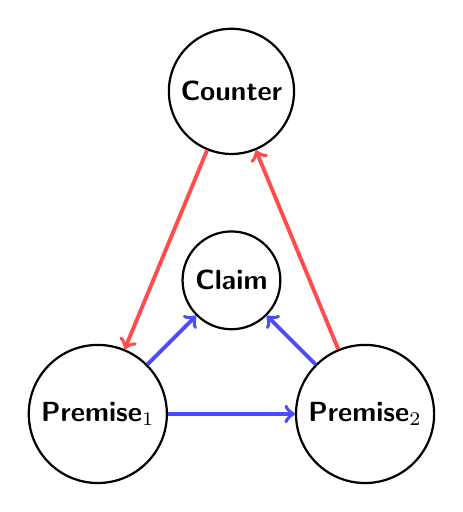
\begin{tikzpicture}[node distance=2.4cm]
        \tikzset{
            arg/.style={draw,circle,thick,minimum size=34pt,font=\sffamily\bfseries},
            support/.style={->, line width=1.4pt, color=blue!70},
            defeat/.style={->, line width=1.4pt, color=red!70}
        }
        \node[arg] (a) {Claim};
        \node[arg] (b) [below left of=a] {Premise$_1$};
        \node[arg] (c) [below right of=a] {Premise$_2$};
        \node[arg] (d) [above of=a] {Counter};
        \draw[support] (b) -- (a);
        \draw[support] (c) -- (a);
        \draw[support] (b) -- (c);
        \draw[defeat] (d) -- (b);
        \draw[defeat] (c) -- (d);
    \end{tikzpicture}
    \caption{Illustrative bipolar argumentation fragment with
             mutual support and derived defeat chains.}
    \label{fig:baf}
\end{figure}

Encoding a BAF in PASP lets us reason about accepted arguments under
probabilistic stable-model semantics while accounting for uncertainty in the
edges or their textual evidence.

\subsection{Knowledge Compilation}

Once the PASP program is grounded, we apply Clark's completion and generate a
structured circuit that satisfies the properties required for tractable 2AMC
inference.

\subsubsection{Clark's Completion and CNF Generation}

In order to obtain a propositional theory equivalent to the stable-model
semantics of the grounded program, we first apply Clark's completion
\citep{clark1978negation}. For normal programs, the Clark's completion equates
each atom with the disjunction of the bodies of the rules that derive it. For
disjunctive programs we obtain

\begin{equation}
    \textsc{Clark}(P) = \bigwedge_{a \in \mathcal{A}(P)}
    \left[a \iff \bigvee_{r \in \mathcal{R}(P,a)}
    \bigwedge_{b \in \mathrm{body}(r)} b
    \bigwedge_{a' \in \mathrm{head}(r) \setminus \{a\}} \neg a'
    \right],
    \label{eq:clark_completion_disjunctive}
\end{equation}
\noindent which yields a conjunctive normal form (CNF) after distributing
conjunctions and disjunctions over the finite grounding. Loop formulas
supplement the completion to eliminate unsupported models, guaranteeing
equivalence with the stable-model semantics \citep{lin2004assat,
eiter2009answer}. Recent analyses tighten this translation by bounding the
number of auxiliary variables introduced during completion, which is crucial for
predictable compilation cost \citep{EITER2024104109}.

\subsubsection{Circuits}
\label{sec:structured-circuits}

For the purposes of this work, Logic circuits are directed acyclic graphs that
represent Boolean functions through internal AND and OR nodes, with literals
labelling the leaves. This family of circuits are often called Negation Normal
Form (NNF) circuits \citep{darwiche2002knowledge}, and there are two key
approaches to using them for representing complex boolean formulas: top-down
compilation, which first translates the formula into a specific normal form
(e.g., CNF) and then compiles it into a circuit; and bottom-up compilation,
which constructs the circuit directly from the formula using a set of
compilation rules (by applying operations such as conjunction, disjunction, and
negation).

To support efficient 2AMC inference, we require circuits that satisfy three main
properties that make algebraic model counting tractable
\citep{Darwiche_2002, darwiche2011sdd}:
\begin{itemize}
    \item \textbf{Decomposability}: sub-circuits combined by a product node refer
          to disjoint sets of variables.
    \item \textbf{Determinism}: the children of a sum node are mutually
          exclusive, preventing double counting.
    \item \textbf{Smoothness}: the children of a sum node mention the same
          variables, enabling weight sharing and differentiation.
\end{itemize}

\begin{figure}[ht]
    \centering
    \begin{tikzpicture}[scale=1.05, every node/.style={font=\small}]
        \tikzset{
            sum/.style={draw,circle,thick,line width=1pt,inner sep=3pt,color=cyan!70!black},
            and/.style={draw,circle,thick,line width=1pt,inner sep=3pt,color=orange!80!black},
            lit/.style={font=\small\ttfamily}
        }
        \node[sum] (root) at (0,0) {$+$};
        \node[and] (and1) at (-2,-1.6) {$\times$};
        \node[and] (and2) at (2,-1.6) {$\times$};
        \node[sum] (sum1) at (-3.4,-3.2) {$+$};
        \node[lit] (litb) at (-0.6,-3.2) {$b$};
        \node[lit] (lita) at (-4.5,-4.8) {$a$};
        \node[lit] (litna) at (-2.3,-4.8) {$\neg a$};
        \node[lit] (litc) at (1.2,-3.2) {$a$};
        \node[lit] (litnb) at (3.0,-3.2) {$\neg b$};
        \draw (root) -- (and1);
        \draw (root) -- (and2);
        \draw (and1) -- (sum1);
        \draw (and1) -- (litb);
        \draw (sum1) -- (lita);
        \draw (sum1) -- (litna);
        \draw (and2) -- (litc);
        \draw (and2) -- (litnb);
    \end{tikzpicture}
    \caption{Smooth, decomposable, and deterministic circuit fragment used for
             PASP inference.}
    \label{fig:structured-circuit}
\end{figure}

Circuits satisfying these properties belong to the sd-DNNF class (smooth,
deterministic, decomposable negation normal form). State-of-the-art compilers
such as \textsc{C2D}, \textsc{D4}, and \textsc{SharpSAT-TD} can target this
class while preserving the structural guarantees required for efficient 2AMC
inference \citep{EITER2024104109}. Their output supports on-the-fly evaluation
of credal and \textsc{MaxEnt} semantics through algebraic model counting
\citep{wang2025}. Moreover, the recent translation scheme of
\citet{maene2024klay} converts logic circuits into tensor-based representations
compatible with automatic differentiation frameworks such as PyTorch or JAX,
enabling gradient-based learning over the compiled model.

\section{Experimental Results}
\label{sec:experimental-outlook}

The experimental section of the dissertation will benchmark the proposed
pipeline against established sd-DNNF compilers. We plan to evaluate
\textsc{C2D}, \textsc{D4}, and \textsc{SharpSAT-TD}, three top-down compilers
adapted by \citep{EITER2024104109} in order to handle the necessary constraints
for tractable PASP inference as 2AMC problem \citep{wang2025}. The workloads
will include the an argumentation program family, which captures the
argumentation instances that motivated our pipeline.

First, we describe the experimental pipeline that will be used to evaluate the
selected knowledge compilers on argumentation mining instances. This outlook
clarifies that the compiled circuits will be assessed mainly for
compilation efficiency, as compiled circuits can be reused for multiple
inference tasks during neuro-symbolic learning. Then, we discuss the expected
outcomes of the experiments, focusing on the research question that the
evaluation aims to address. Finally, we analyse the experimental results
obtained from running the proposed pipeline with the selected compilers in
argumenatation mining instances ranging from 3 nodes to 50 nodes (a large scale
when considering the complexity of exact neuro-symbolic inference).

\subsection{Experimental Outlook}

\paragraph{Program listing.} The generator produces instantiations of the
following ungrounded PASP template, which encodes argumentation constraints
before grounding:

\begin{minted}[fontsize=\small,breaklines]{prolog}
% Domain and probabilistic choices over components
node(ARG) :- argument(ARG).
0.5::aux_component(ARG,0) :- node(ARG).
0.5::aux_component(ARG,1) :- node(ARG).

component(ARG,0) :- aux_component(ARG,0).
component(ARG,1) :- aux_component(ARG,1), not aux_component(ARG,0).
component(ARG,2) :- node(ARG), not aux_component(ARG,1), not aux_component(ARG,0).

% Probabilistic relations between distinct arguments
0.5::relation(SRC,DST) :- node(SRC), node(DST), SRC != DST.

% Stratification constraints
fail :- node(SRC), node(DST), SRC != DST, component(SRC,2), not relation(SRC,DST).
fail :- node(SRC), node(DST), SRC != DST, component(SRC,1), not component(DST,2), not relation(SRC,DST).
fail :- node(SRC), node(DST), SRC != DST, component(SRC,0), component(DST,2), not relation(SRC,DST).
\end{minted}

\paragraph{Grounding.} The grounding step instantiates the above program over a
set of arguments provided as input. For an input size of $n$ arguments, the
grounded program contains $3n$ probabilistic facts for the components and
$n(n-1)/2$ probabilistic facts for the relations, resulting in a total of
$3n + n(n-1)/2$ probabilistic facts. Note that the number of rules in the
grounded program grows quadratically with $n$ due to the pairwise relations
between arguments. In order to compute such groundings, we use \emph{clingo},
the state-of-the-art ASP grounder \citep{gebser2014clingo}.

\paragraph{Knowledge compilation.} Given the grounded program, we apply Clark's
completion and generate the corresponding CNF with loop formulas, by following
the algorithm present in \citep{lee2003loop} (another possible approach would be
to follow the algorithm present in \citep{EITER2024104109}, which uses the
cycle-breaking method from \citep{eiter2021treewidth}). The resulting CNF is
then fed to the selected knowledge compilers, which produce sd-DNNF circuits that
support efficient 2AMC inference.

\paragraph{Evaluation metrics.} We will assess the performance of the knowledge
compilers along two axes: compilation time and circuit size. Compilation time
measures the duration required by each compiler to process the CNF and produce
the sd-DNNF circuit. Circuit size is evaluated in terms of the number of nodes
and edges in the resulting circuit, as well as the memory footprint. These
metrics provide insights into the efficiency and scalability of each compiler
when handling the argumentation instances generated by our program template.

\paragraph{Neuro-Symbolic Learning} Given that the circuits produced by the
compilers support efficient 2AMC inference, they do not need to be recompiled
when evidence or queries change, i.e. then the probabilities estimated by neural
components vary during training. This property enables the integration of the
compiled circuits into end-to-end neuro-symbolic learning loops, where neural
networks provide probabilistic inputs to the PASP program, and gradients can be
backpropagated through the circuit to update the neural parameters. We plan to
explore this integration in future work, building upon the tensor-based circuit
representations introduced by \citet{maene2024klay}.

\subsection{Expected Outcomes}
\label{subsec:expected-outcomes}

The only variable factor in the proposed pipeline is the knowledge compiler, as
the grounding and CNF generation steps are deterministic and the PASP program is
fixed. Therefore, we expect the experimental evaluation to reveal differences in
compilation time and circuit size among the selected compilers. These differences
will inform the choice of the most suitable compiler for integrating into
neuro-symbolic learning loops for argumentation mining. Ultimately, the goal is
to identify a compilation strategy that balances efficiency and scalability,
enabling practical applications of probabilistic argumentation mining in
real-world scenarios.

Therefore, the only applicable research question for this experimental outlook
is: which knowledge compiler among \textsc{C2D}, \textsc{D4}, and
\textsc{SharpSAT-TD} produces the most efficient sd-DNNF circuits for
argumentation instances, in terms of compilation time and circuit size?

Given the results from \citep{EITER2024104109} on a variety of PASP programs,
we expect \textsc{SharpSAT-TD} to outperform the other two compilers in both
compilation time and circuit size, due to its advanced top-down compilation
techniques, while \textsc{C2D} and \textsc{D4} may exhibit longer compilation
times and larger circuits. However, the actual performance may vary depending on
the specific structure of the argumentation instances generated by our program
template.

\subsection{Empirical Analysis}
\label{subsec:empirical-analysis}

Still pending (results are stored in my desktop and the energy crysis is
delaying acess to the CSVs containing the data).
